%%
%% Automatically generated file from DocOnce source
%% (https://github.com/hplgit/doconce/)
%%
%%


%-------------------- begin preamble ----------------------

\documentclass[%
twoside,                 % oneside: electronic viewing, twoside: printing
final,                   % or draft (marks overfull hboxes, figures with paths)
10pt]{article}

\listfiles               % print all files needed to compile this document

\usepackage{relsize,makeidx,color,setspace,amsmath,amsfonts}
\usepackage[table]{xcolor}
\usepackage{bm,microtype}

\usepackage{graphicx}

\usepackage{fancyvrb} % packages needed for verbatim environments

\usepackage{minted}
\usemintedstyle{default}

\usepackage[T1]{fontenc}
%\usepackage[latin1]{inputenc}
\usepackage{ucs}
\usepackage[utf8x]{inputenc}

\usepackage{lmodern}         % Latin Modern fonts derived from Computer Modern

% Hyperlinks in PDF:
\definecolor{linkcolor}{rgb}{0,0,0.4}
\usepackage{hyperref}
\hypersetup{
    breaklinks=true,
    colorlinks=true,
    linkcolor=linkcolor,
    urlcolor=linkcolor,
    citecolor=black,
    filecolor=black,
    %filecolor=blue,
    pdfmenubar=true,
    pdftoolbar=true,
    bookmarksdepth=3   % Uncomment (and tweak) for PDF bookmarks with more levels than the TOC
    }
%\hyperbaseurl{}   % hyperlinks are relative to this root

\setcounter{tocdepth}{2}  % number chapter, section, subsection

% Tricks for having figures close to where they are defined:
% 1. define less restrictive rules for where to put figures
\setcounter{topnumber}{2}
\setcounter{bottomnumber}{2}
\setcounter{totalnumber}{4}
\renewcommand{\topfraction}{0.85}
\renewcommand{\bottomfraction}{0.85}
\renewcommand{\textfraction}{0.15}
\renewcommand{\floatpagefraction}{0.7}
% 2. ensure all figures are flushed before next section
\usepackage[section]{placeins}
% 3. enable begin{figure}[H] (often leads to ugly pagebreaks)
%\usepackage{float}\restylefloat{figure}

\usepackage[framemethod=TikZ]{mdframed}

% --- begin definitions of admonition environments ---

% --- end of definitions of admonition environments ---

% prevent orhpans and widows
\clubpenalty = 10000
\widowpenalty = 10000

\newenvironment{doconceexercise}{}{}
\newcounter{doconceexercisecounter}


% ------ header in subexercises ------
%\newcommand{\subex}[1]{\paragraph{#1}}
%\newcommand{\subex}[1]{\par\vspace{1.7mm}\noindent{\bf #1}\ \ }
\makeatletter
% 1.5ex is the spacing above the header, 0.5em the spacing after subex title
\newcommand\subex{\@startsection*{paragraph}{4}{\z@}%
                  {1.5ex\@plus1ex \@minus.2ex}%
                  {-0.5em}%
                  {\normalfont\normalsize\bfseries}}
\makeatother


% --- end of standard preamble for documents ---


% insert custom LaTeX commands...

\raggedbottom
\makeindex

%-------------------- end preamble ----------------------

\begin{document}



% ------------------- main content ----------------------



% ----------------- title -------------------------

\thispagestyle{empty}

\begin{center}
{\LARGE\bf
\begin{spacing}{1.25}
Integrating computations, mathematics, physics and chemistry in undergraduate biology programs
\end{spacing}
}
\end{center}

% ----------------- author(s) -------------------------

\begin{center}
{\bf Morten Hjorth-Jensen${}^{1, 2}$} \\ [0mm]
\end{center}

    
\begin{center}
{\bf Hans Petter Langtangen${}^{3, 4}$} \\ [0mm]
\end{center}

    \begin{center}
% List of all institutions:
\centerline{{\small ${}^1$Dept.~of Physics, UiO}}
\centerline{{\small ${}^2$Dept.~of Physics, Michigan State University}}
\centerline{{\small ${}^3$Dept.~of Informatics, UiO}}
\centerline{{\small ${}^4$Center for Biomedical Computing, Simula}}
\end{center}
    
% ----------------- end author(s) -------------------------

\begin{center} % date
Feb 26, 2015
\end{center}

\vspace{1cm}


% !split
\subsection*{Overarching questions}

% !bpop

% --- begin paragraph admon ---
\paragraph{Which skills are needed by MSc candidates in biology?}
There is new demand for more

\begin{itemize}
  \item quantitative methods {\&} reasoning

  \item understanding data and phenomena via models

  \item creating \emph{in silico} virtual labs
\end{itemize}

\noindent
% --- end paragraph admon ---


% !epop

% !bpop

% --- begin paragraph admon ---
\paragraph{Challenge:}
How to integrate such computing-based activities in the bachelor programs
when the students are \emph{not} interested in mathematics, physics, and
programming?
% --- end paragraph admon ---


% !epop

% !split
\subsection*{How to teach computing in biology?}

% !bpop

% --- begin paragraph admon ---
\paragraph{}
Do we need to still follow the tradition and teach mathematics, physics, computations, chemistry, etc. in separate discipline-specific courses?

\begin{itemize}
  \item Uninteresting to first study tools when you want to study biology

  \item Little understanding of what the tools are good for

  \item Minor utilization of tools later in biology
\end{itemize}

\noindent
% --- end paragraph admon ---


% !epop

% !bpop

% --- begin paragraph admon ---
\paragraph{It's time for new thinking:}
\begin{itemize}
  \item Just-in-time teaching: teach tools \emph{when needed}

  \item Teach tools in the \emph{context of biology}

  \item Emphasize development of \emph{intuition and understanding}

  \item Base learning of the students' own \emph{explorations in biology projects}

  \item Integrate lab work with computing tools
\end{itemize}

\noindent
% --- end paragraph admon ---


% !epop



% !split
\subsection*{Pilot project: Oct 2014 - Oct 2015}


% --- begin paragraph admon ---
\paragraph{}
\begin{itemize}
 \item Form a project team of dedicated CSE+IBV people and  PhD students

 \item Develop a pedagogical framework

 \item CSE+IBV people identify a set of possible examples

 \item PhD students work closely with CSE+IBV people to find data,
   define models, and write documents

 \item Fall 2015: intro course in computing and programming for IBV teachers, using selected examples

 \item Educational workshop at IBV:
\begin{itemize}

   \item Present results from the project

   \item Discuss how and where to implement examples in BIOxxxx courses

\end{itemize}

\noindent
 \item Fall 2016: First integration of computing in courses
\end{itemize}

\noindent
% --- end paragraph admon ---




% !split
\subsection*{The pedagogical framework}


% --- begin paragraph admon ---
\paragraph{Aim: Develop intuition about the scientific method.}
\begin{itemize}
 \item Method: case-based learning

 \item Coherent problem solving \emph{in biology} by integrating
   mathematics, programming, physics/chemistry, ...

 \item Starting point: data from lab or field experiments

 \item Visualize data

 \item Derive computational models directly from mathematical/intuitive \emph{reasoning}

 \item Program model(s), fit parameters, compare with data

 \item Develop intuition and understanding based on
\begin{itemize}

  \item the principles behind the model

  \item exploration of the model (``what if'')

  \item prediction of new experiments
\end{itemize}

\noindent
\end{itemize}

\noindent
% --- end paragraph admon ---



% !split
\subsection*{Example 1: ecoli lab experiment}


% --- begin paragraph admon ---
\paragraph{}
Observations of no of bacteria vs time in seconds,
stored in Excel and written to a CVS file:

\begin{minted}[fontsize=\fontsize{9pt}{9pt},linenos=false,mathescape,baselinestretch=1.0,fontfamily=tt,xleftmargin=7mm]{text}
0,100
600,140
1200,250
1800,360
2400,480
3000,820
3600,1300
4200,1700
4800,2900
5400,3900
6000,7000
\end{minted}
% --- end paragraph admon ---



% !split
\subsection*{Visualize data}


% --- begin paragraph admon ---
\paragraph{}
\begin{itemize}
 \item Meet a text editor and a terminal window

 \item Very basic Unix
\end{itemize}

\noindent
First program:

\begin{minted}[fontsize=\fontsize{9pt}{9pt},linenos=false,mathescape,baselinestretch=1.0,fontfamily=tt,xleftmargin=7mm]{python}
t = [0, 600, 1200, 1800, 2400, 3000, 3600,
     4200, 4800, 5400, 6000]
N = [100, 140, 250, 360, 480, 820, 1300, 1700, 2900, 3900, 7000]
import matplotlib.pyplot as plt
plt.plot(t, N, 'ro')
plt.xlabel('t [s]')
plt.ylabel('N')
plt.show()
\end{minted}
% --- end paragraph admon ---




% !split
\subsection*{Concepts must be introduced implicitly in a structured way}


% --- begin paragraph admon ---
\paragraph{Warning.}
\begin{itemize}
 \item Always identify new concepts

 \item Train new concepts in simplified (``trivial'') problems
\end{itemize}

\noindent
% --- end paragraph admon ---




% --- begin paragraph admon ---
\paragraph{Concepts in the previous example:}
\begin{itemize}
 \item Lists or arrays of numbers

 \item Plotting commands

 \item Curve = function of time
\end{itemize}

\noindent
% --- end paragraph admon ---




% --- begin paragraph admon ---
\paragraph{Notice:}
The concept of a continuous function $N(t)$ is not necessary,
just straight lines between discrete points on a curve.
% --- end paragraph admon ---



% !split
\subsection*{Read data from file}


% --- begin paragraph admon ---
\paragraph{}
\begin{minted}[fontsize=\fontsize{9pt}{9pt},linenos=false,mathescape,baselinestretch=1.0,fontfamily=tt,xleftmargin=7mm]{python}
import numpy as np
data = np.loadtxt('ecoli.csv', delimiter=',')
print data  # look at the format
t = data[:,0]
N = data[:,1]
import matplotlib.pyplot as plt
plt.plot(t, N, 'ro')
plt.xlabel('t [s]')
plt.ylabel('N')
plt.show()
\end{minted}
% --- end paragraph admon ---




% --- begin paragraph admon ---
\paragraph{Typical pattern:}
The population grows faster and faster. Why? Is there an
underlying (general) mechanism?
% --- end paragraph admon ---



% !split
\subsection*{Lab journal}


% --- begin paragraph admon ---
\paragraph{}
Use IPython notebook as lab journal.
% --- end paragraph admon ---




% !split
\subsection*{How can we reason about the process?}

% \href{{http://www.zo.utexas.edu/courses/Thoc/PopGrowth.html}}{\nolinkurl{http://www.zo.utexas.edu/courses/Thoc/PopGrowth.html}}


% --- begin paragraph admon ---
\paragraph{}
% !bpop
\begin{enumerate}
\item Cells divide after $T$ seconds on average (one generation)

\item $2N$ celles divide into twice as many new cells $\Delta N$ in a time
   interval $\Delta t$ as $N$ cells would: $\Delta N \propto N$

\item $N$ cells result in twice as many new individuals $\Delta N$ in
   time $2\Delta t$ as in time $\Delta t$: $\Delta N \propto\Delta t$

\item Same proportionality wrt death (repeat reasoning)

\item Proposed model: $\Delta N = b\Delta t N - d\Delta tN$ for some unknown
   constants $b$ (births) and $d$ (deaths)

\item Describe evolution in discrete time: $t_n=n\Delta t$

\item Program-friendly notation: $N$ at $t_n$ is $N^n$

\item Math model: $N^{n+1} = N^n + r\Delta t\, N$ (with $\ r=b-d$)

\item Program model: \Verb!N[n+1] = N[n] + r*dt*N[n]!
\end{enumerate}

\noindent
% !epop
% --- end paragraph admon ---



% !split
\subsection*{The first simple program}


% --- begin paragraph admon ---
\paragraph{}
Let us solve the difference equation in as simple way as possible,
just to train some programming: $r=1.5$, $N^0=1$, $\Delta t=0.5$

\begin{minted}[fontsize=\fontsize{9pt}{9pt},linenos=false,mathescape,baselinestretch=1.0,fontfamily=tt,xleftmargin=7mm]{python}
import numpy as np

t = np.linspace(0, 10, 21)  # 20 intervals in [0, 10]
dt = t[1] - t[0]
N = np.zeros(t.size)

N[0] = 1
r = 0.5

for n in range(0, N.size-1, 1):
    N[n+1] = N[n] + r*dt*N[n]
    print 'N[%d]=%.1f' % (n+1, N[n+1])
\end{minted}
% --- end paragraph admon ---



% !split
\subsection*{The output}

\begin{Verbatim}[numbers=none,fontsize=\fontsize{9pt}{9pt},baselinestretch=0.95]
N[1]=1.2
N[2]=1.6
N[3]=2.0
N[4]=2.4
N[5]=3.1
N[6]=3.8
N[7]=4.8
N[8]=6.0
N[9]=7.5
N[10]=9.3
N[11]=11.6
N[12]=14.6
N[13]=18.2
N[14]=22.7
N[15]=28.4
N[16]=35.5
N[17]=44.4
N[18]=55.5
N[19]=69.4
N[20]=86.7
\end{Verbatim}

% !split
\subsection*{Parameter estimation}


% --- begin paragraph admon ---
\paragraph{}
\begin{itemize}
 \item We do not know $r$

 \item How can we estimate $r$ from data?
\end{itemize}

\noindent
We can use the difference equation with the experimental data

\[ N^{n+1} = N^n + r\Delta t N^n\]
Say $N^{n+1}$ and $N^n$ are known from data, solve wrt $r$:

\[ r = \frac{N^{n+1}-N^n}{N^n\Delta t} \]

Use experimental data in the fraction, say $t_1=600$, $t_2=1200$,
$N^1=140$, $N^2=250$: $r=0.0013$.
% --- end paragraph admon ---




% --- begin paragraph admon ---
\paragraph{More sophisticated methods.}
Can do a nonlinear least squares parameter fit, but that is
too advanced at this stage.
% --- end paragraph admon ---



% !split
\subsection*{A program relevant for the biological problem}

% exact r = 0.000694


% --- begin paragraph admon ---
\paragraph{}
\begin{minted}[fontsize=\fontsize{9pt}{9pt},linenos=false,mathescape,baselinestretch=1.0,fontfamily=tt,xleftmargin=7mm]{python}
import numpy as np

# Estimate r
data = np.loadtxt('ecoli.csv', delimiter=',')
t_e = data[:,0]
N_e = data[:,1]
i = 2  # Data point (i,i+1) used to estimate r
r = (N_e[i+1] - N_e[i])/(N_e[i]*(t_e[i+1] - t_e[i]))
print 'Estimated r=%.5f' % r
# Can experiment with r values and see if the model can
# match the data better

T = 1200     # cell can divide after T sec
t_max = 5*T  # 5 generations in experiment
t = np.linspace(0, t_max, 1000)
dt = t[1] - t[0]
N = np.zeros(t.size)

N[0] = 100
for n in range(0, len(t)-1, 1):
    N[n+1] = N[n] + r*dt*N[n]

import matplotlib.pyplot as plt
plt.plot(t, N, 'r-', t_e, N_e, 'bo')
plt.xlabel('time [s]');  plt.ylabel('N')
plt.legend(['model', 'experiment'], loc='upper left')
plt.show()
\end{minted}

Change \Verb!r! in the program and play around to make a better fit!
% --- end paragraph admon ---



% !split
\subsection*{Discuss the nature of such a model}


% --- begin paragraph admon ---
\paragraph{}
\begin{itemize}
 \item Write up all the biological factors that influence the
   population size of bacteria

 \item Understand that all such effects are merged into one parameter $r$

 \item Understand that the reasoning must be the same whether we
   have bacteria, animals or humans - this is a generic model!\\
   (even the interest rate in a bank follows the same model)
\end{itemize}

\noindent
% --- end paragraph admon ---



% !split
\subsection*{Discuss the limitations of such a model}


% --- begin paragraph admon ---
\paragraph{}
\begin{itemize}
 \item How many bacteria in the lab after one month?

 \item Growth is restricted by environmental resources!

 \item Fix the model (logistic growth)

 \item Is the logistic model appropriate for a lab experiment?

 \item Find data to support the logistic model \\
   (it's a \emph{very} simple model)
\end{itemize}

\noindent
% --- end paragraph admon ---




% !split
\subsection*{The pedagogical template (to be iterated!)}


% --- begin paragraph admon ---
\paragraph{}
\begin{itemize}
 \item Start with a real biological problem

 \item Be careful with too many new concepts

 \item Workflow:
\begin{itemize}

  \item data

  \item visualization

  \item patterns

  \item modeling (\emph{discrete})

  \item programming

  \item testing

  \item parameter estimation (difficult)

  \item validation

  \item prediction

\end{itemize}

\noindent
 \item Make many small exercises that train the new concepts

 \item Repeat the case in a way that makes a complete understanding
\end{itemize}

\noindent
% --- end paragraph admon ---



% !split
\subsection*{Technology for documenting cases}


% --- begin paragraph admon ---
\paragraph{}
\begin{itemize}
 \item Documentation: slides in the doconce format with extra notes\\
   (can compile with/without notes)

 \item Realistic goal: write out the slides for a gentle book on biocomputing examples

 \item The biological case is in a separate file that the students can work
   with as an IPython notebook

 \item Problem: not much basic literature exists

 \item Cases must be linked in a learning graph:\\
   \emph{I want to do nerve cell modeling, but how to progress to this stage?}

 \item Make a list of concepts and where concepts are trained

 \item Think of each case as a \emph{separate module}
\end{itemize}

\noindent
% --- end paragraph admon ---



% !split
\subsection*{Immediate tasks}


% --- begin paragraph admon ---
\paragraph{}
\begin{itemize}
 \item Find a good bacteria growth lab example - do the first example

 \item Alternative model: random 2D walk, people meet and make new individuals

 \item Predator-pray model: any field experiment to build?

 \item Experiments based on technology: imaging, sensors, ...

 \item Disease modeling coupled to data

 \item Predator-pray with disease

 \item Bioinformatics cases and programming

 \item ...
\end{itemize}

\noindent
% --- end paragraph admon ---



% !split
\subsection*{Adding model complexity: Predator-Prey model from ecology}


% --- begin paragraph admon ---
\paragraph{}
The population dynamics of a simple predator-prey system is a
classical example shown in many biology textbooks when ecological
systems are discussed. The system contains all elements of the
scientific method:

\begin{itemize}
 \item The set up of a specific hypothesis combined with

 \item the experimental methods needed (one can study existing data or perform experiments)

 \item analyzing and interpreting the data and performing further experiments if needed

 \item trying to extract general behaviors and extract eventual laws or patterns

 \item develop mathematical relations for the uncovered regularities/laws and test these by performing new experiments
\end{itemize}

\noindent
% --- end paragraph admon ---




% !split
\subsection*{Case study from Hudson bay}


% --- begin paragraph admon ---
\paragraph{}
Lots of data about populations of hares and lynx collected from furs in Hudson Bay, Canada, are available. It is known that the populations oscillate. Why?
We shall demonstrate the scientific method by

\begin{enumerate}
\item plotting the data

\item derive a simple model for the population dynamics

\item (fitting parameters in the model to the data)

\item using the model predict the evolution other predator-pray systems
\end{enumerate}

\noindent
% --- end paragraph admon ---



% !split
\subsection*{Hudson bay data}



% --- begin paragraph admon ---
\paragraph{}


\begin{quote}
\begin{tabular}{lrr}
\hline
\multicolumn{1}{c}{ Year } & \multicolumn{1}{c}{ Hares (x1000) } & \multicolumn{1}{c}{ Lynx (x1000) } \\
\hline
1900 & 30.0          & 4.0          \\
1901 & 47.2          & 6.1          \\
1902 & 70.2          & 9.8          \\
1903 & 77.4          & 35.2         \\
1904 & 36.3          & 59.4         \\
1905 & 20.6          & 41.7         \\
1906 & 18.1          & 19.0         \\
1907 & 21.4          & 13.0         \\
1908 & 22.0          & 8.3          \\
1909 & 25.4          & 9.1          \\
1910 & 27.1          & 7.4          \\
1911 & 40.3          & 8.0          \\
1912 & 57            & 12.3         \\
1913 & 76.6          & 19.5         \\
1914 & 52.3          & 45.7         \\
1915 & 19.5          & 51.1         \\
1916 & 11.2          & 29.7         \\
1917 & 7.6           & 15.8         \\
1918 & 14.6          & 9.7          \\
1919 & 16.2          & 10.1         \\
1920 & 24.7          & 8.6          \\
\hline
\end{tabular}
\end{quote}

\noindent
% --- end paragraph admon ---





% !split
\subsection*{Plotting the data}


% --- begin paragraph admon ---
\paragraph{}
\begin{minted}[fontsize=\fontsize{9pt}{9pt},linenos=false,mathescape,baselinestretch=1.0,fontfamily=tt,xleftmargin=7mm]{python}
import numpy as np
from  matplotlib import pyplot as plt

# Load in data file
data = np.loadtxt('Hudson_Bay.dat', delimiter=',', skiprows=1)
# Make arrays containing x-axis and hares and lynx populations
year = data[:,0]
hares = data[:,1]
lynx = data[:,2]

plt.plot(year, hares ,'b-+', year, lynx, 'r-o')
plt.axis([1900,1920,0, 100.0])
plt.xlabel(r'Year')
plt.ylabel(r'Numbers of hares and lynx ')
plt.legend(('Hares','Lynx'), loc='upper right')
plt.title(r'Population of hares and lynx from 1900-1920 (x1000)}')
plt.savefig('Hudson_Bay_data.pdf')
plt.savefig('Hudson_Bay_data.png')
plt.show()
\end{minted}
% --- end paragraph admon ---



% !split
\subsection*{Hares and lynx in Hudson bay from 1900 to 1920}



% inline figure
\centerline{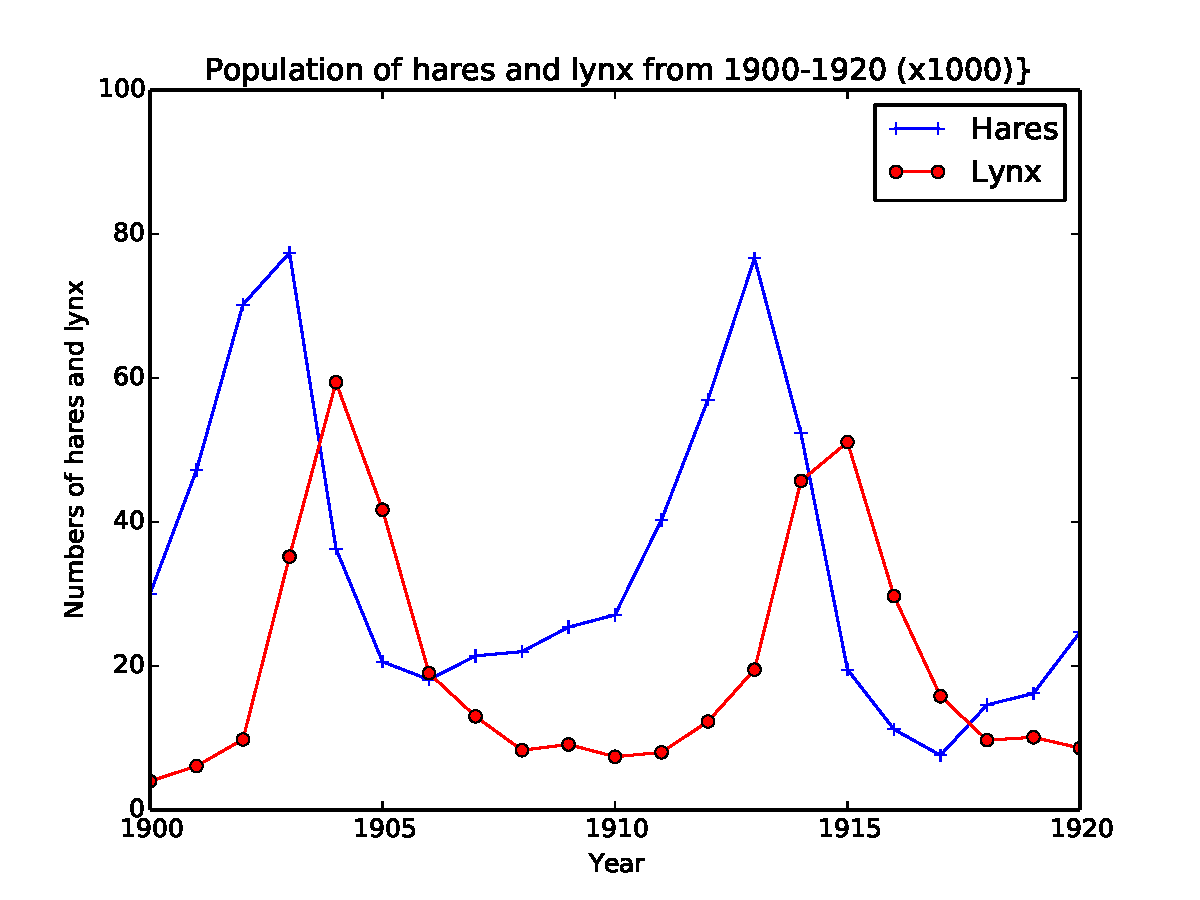
\includegraphics[width=0.9\linewidth]{fig/Hudson_Bay_data.pdf}}




% !split
\subsection*{Why now create a computer model for the hare and lynx populations?}

% --- begin paragraph admon ---
\paragraph{}
\begin{itemize}
 \item We see oscillations in the data

 \item What causes cycles to slow or speed up?

 \item What affects the amplitude of the oscillation or do you expect to see the oscillations damp to a stable equilibrium?

 \item With a model we can better \emph{understand the data}

 \item More important: we can understand the ecology dynamics of
   predator-pray populations
\end{itemize}

\noindent
% --- end paragraph admon ---




% !split
\subsection*{The traditional (top-down) approach}


% --- begin paragraph admon ---
\paragraph{}
The classical way (in all books) is to present the Lotka-Volterra equations:

\begin{align*}
\frac{dH}{dt} &= H(a - b L)\\ 
\frac{dL}{dt} &= - L(d - c  H)
\end{align*}

Here,

\begin{itemize}
 \item $H$ is the number of preys

 \item $L$ the number of predators

 \item $a$, $b$, $d$, $c$ are parameters
\end{itemize}

\noindent
Most books quickly establish the model and then use considerable space on
discussing the qualitative properties of this \emph{nonlinear system of
ODEs} (which cannot be solved)
% --- end paragraph admon ---




% !split
\subsection*{The ``new'' discrete bottom-up approach}


% --- begin paragraph admon ---
\paragraph{The bottom-up approach.}
% !bpop
\begin{itemize}
 \item Start with experimental data and discuss the methods which have been used to collect the data, the assumptions, the electronic devices, the aims etc. That is, expose the students to the theory and assumptions behind the data that have been collected and motivate for the scientific method.

 \item Where appropriate the students should do the experiment(s) needed to collect the data.

 \item The first programming tasks are to read and visualize the data to see if there are patterns or regularities. This strengthens a research-driven intuition.

 \item Now we want to increase the understanding through modeling.

 \item Most of the biology lies in the \emph{derivation} of the model. We shall
   focus on an intuitive discrete approach that leads to difference
   equations that can be programmed \emph{and solved} directly.
\end{itemize}

\noindent
% !epop
% --- end paragraph admon ---



% !split
\subsection*{Basic (computer-friendly) mathematics notation}

% --- begin paragraph admon ---
\paragraph{}
\begin{itemize}
 \item Time points: $t_0,t_1,\ldots,t_m$

 \item Uniform distribution of time points: $t_n=n\Delta t$

 \item $H^n$: population of hares at time $t_n$

 \item $L^n$: population of lynx at time $t_n$

 \item We want to model the changes in populations, $\Delta H=H^{n+1}-H^n$
   and $\Delta L=L^{n+1}-L^n$ during a general time interval $[t_{n+1},t_n]$
   of length $\Delta t=t_{n+1}-t_n$
\end{itemize}

\noindent
% --- end paragraph admon ---



% !split
\subsection*{Basic dynamics of the population of hares}


% --- begin paragraph admon ---
\paragraph{}
The population of hares evolves due to births and deaths exactly as a bacteria population:

\[
\Delta H = a \Delta t H^n
\]
However, hares have an additional loss in the population because
they are eaten by lynx.
All the hares and lynx can form
$H\cdot L$ pairs in total. When such pairs meet during a time
interval $\Delta t$, there is some
small probablity that the lynx will eat the hare.
So in fraction $b\Delta t HL$, the lynx eat hares. This
loss of hares and must be accounted for:
subtracted in the equation for hares:

\[ \Delta H = a\Delta t H^n - b \Delta t H^nL^n\]
% --- end paragraph admon ---



% !split
\subsection*{Basic dynamics of the population of lynx}


% --- begin paragraph admon ---
\paragraph{}
We assume that the primary growth for the lynx population depends on sufficient food for raising lynx kittens, which implies an adequate source of nutrients from predation on hares. Thus, the growth of the lynx population does not only depend of how many lynx there are, but on how many hares they can eat.
In a time interval $\Delta t HL$ hares and lynx can meet, and in a
fraction $b\Delta t HL$ the lynx eats the hare. All of this does not
contribute to the growth of lynx, again just a fraction of
$b\Delta t HL$ that we write as
$d\Delta t HL$. In addition, lynx die just as in the population
dynamics with one isolated animal population, leading to a loss
$-c\Delta t L$.
% --- end paragraph admon ---




% --- begin paragraph admon ---
\paragraph{}
The accounting of lynx then looks like
\[ \Delta L = d\Delta t H^nL^n - c\Delta t L^n\]
% --- end paragraph admon ---



% !split
\subsection*{Evolution equations}


% --- begin paragraph admon ---
\paragraph{}
By writing up the definition of $\Delta H$ and $\Delta L$, and putting
all assumed known terms $H^n$ and $L^n$ on the right-hand side, we have

\[ H^{n+1} = H^n + a\Delta t H^n - b\Delta t H^n L^n \]

\[ L^{n+1} = L^n + d\Delta t H^nL^n - c\Delta t L^n \]

Note:

\begin{itemize}
 \item These equations are ready to be implemented!

 \item But to start, we need $H^0$ and $L^0$ \\
   (which we can get from the data)

 \item We also need values for $a$, $b$, $d$, $c$
\end{itemize}

\noindent
% --- end paragraph admon ---



% !split
\subsection*{Adapt the model to the Hudson Bay case}


% --- begin paragraph admon ---
\paragraph{}
\begin{itemize}
 \item As always, models tend to be general - as here, applicable
   to ``all'' predator-pray systems

 \item The critical issue is whether the \emph{interaction} between hares and lynx
   is sufficiently well modeled by $\hbox{const}HL$

 \item The parameters $a$, $b$, $d$, and $c$ must be
   estimated from data

 \item Measure time in years

 \item $t_0=1900$, $t_m=1920$
\end{itemize}

\noindent
% --- end paragraph admon ---



% !split
\subsection*{The program}


% --- begin paragraph admon ---
\paragraph{}
\begin{minted}[fontsize=\fontsize{9pt}{9pt},linenos=false,mathescape,baselinestretch=1.0,fontfamily=tt,xleftmargin=7mm]{python}
import numpy as np
import matplotlib.pyplot as plt

def solver(m, H0, L0, dt, a, b, c, d, t0):
    """Solve the difference equations for H and L over m years
    with time step dt (measured in years."""

    num_intervals = int(m/float(dt))
    t = np.linspace(t0, t0 + m, num_intervals+1)
    H = np.zeros(t.size)
    L = np.zeros(t.size)

    print 'Init:', H0, L0, dt
    H[0] = H0
    L[0] = L0

    for n in range(0, len(t)-1):
        H[n+1] = H[n] + a*dt*H[n] - b*dt*H[n]*L[n]
        L[n+1] = L[n] + d*dt*H[n]*L[n] - c*dt*L[n]
    return H, L, t

# Load in data file
data = np.loadtxt('Hudson_Bay.csv', delimiter=',', skiprows=1)
# Make arrays containing x-axis and hares and lynx populations
t_e = data[:,0]
H_e = data[:,1]
L_e = data[:,2]

# Simulate using the model
H, L, t = solver(m=20, H0=34.91, L0=3.857, dt=0.1,
                 a=0.4807, b=0.02482, c=0.9272, d=0.02756,
                 t0=1900)

# Visualize simulations and data
plt.plot(t_e, H_e, 'b-+', t_e, L_e, 'r-o', t, H, 'm--', t, L, 'k--')
plt.xlabel('Year')
plt.ylabel('Numbers of hares and lynx')
plt.axis([1900, 1920, 0, 140])
plt.title(r'Population of hares and lynx 1900-1920 (x1000)')
plt.legend(('H_e', 'L_e', 'H', 'L'), loc='upper left')
plt.savefig('Hudson_Bay_sim.pdf')
plt.savefig('Hudson_Bay_sim.png')
plt.show()
\end{minted}
% --- end paragraph admon ---



% !split
\subsection*{The plot}



% inline figure
\centerline{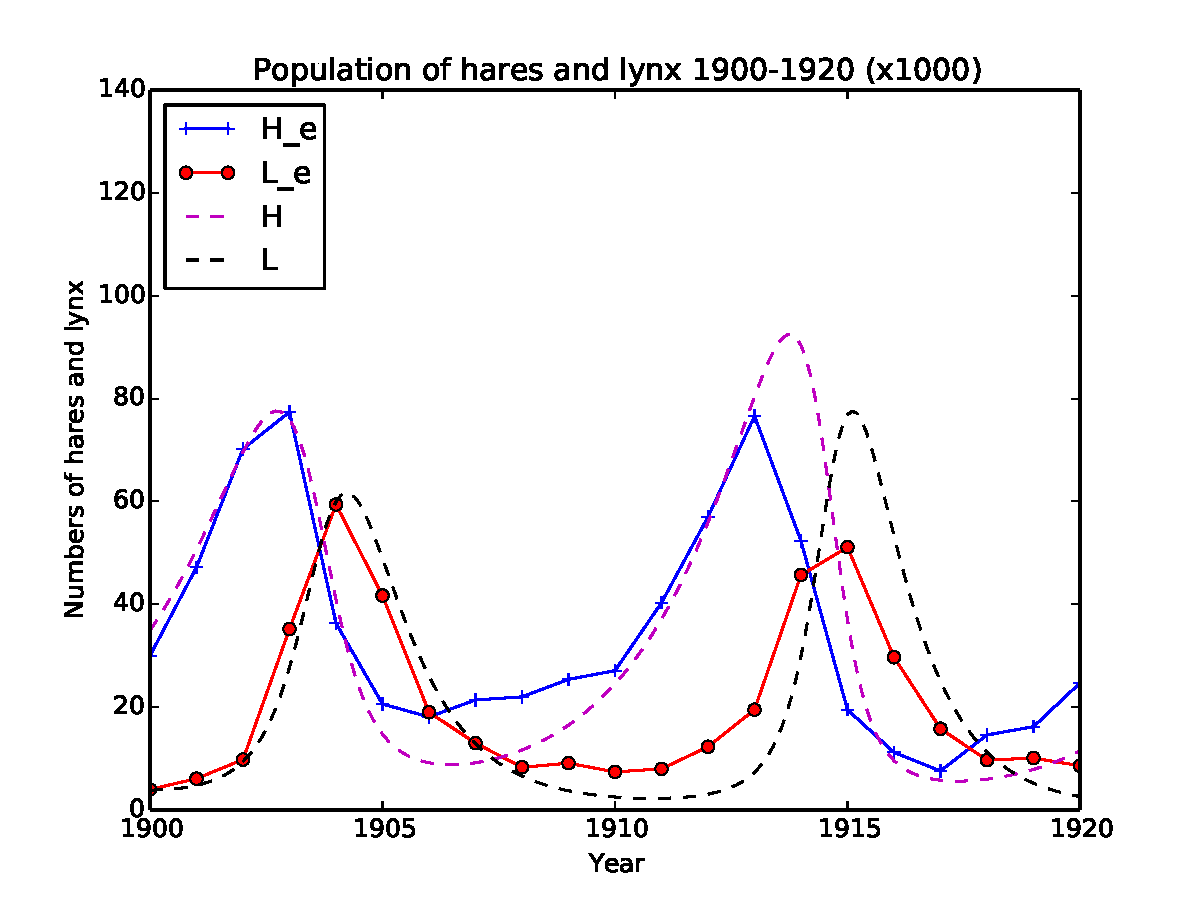
\includegraphics[width=0.9\linewidth]{fig/Hudson_Bay_sim.pdf}}




% !split
\subsection*{Other examples}

% --- begin paragraph admon ---
\paragraph{}
\begin{itemize}
 \item \href{{http://hplgit.github.io/disease-modeling/doc/web/index.html}}{Disease modeling}

 \item Predator-pray with disease

 \item \href{{http://hplgit.github.io/bioinf-py/doc/web/index.html}}{Bioinformatics: searching in strings}

 \item Move from difference equations to differential equations, would this be meaningful? Probably not - it does not give anything in biology before the models are so complex that one needs other things than Forward Euler...
\end{itemize}

\noindent
% --- end paragraph admon ---



% ------------------- end of main content ---------------


\printindex

\end{document}

